% Options for packages loaded elsewhere
\PassOptionsToPackage{unicode}{hyperref}
\PassOptionsToPackage{hyphens}{url}
%
\documentclass[
]{article}
\usepackage{amsmath,amssymb}
\usepackage{iftex}
\ifPDFTeX
  \usepackage[T1]{fontenc}
  \usepackage[utf8]{inputenc}
  \usepackage{textcomp} % provide euro and other symbols
\else % if luatex or xetex
  \usepackage{unicode-math} % this also loads fontspec
  \defaultfontfeatures{Scale=MatchLowercase}
  \defaultfontfeatures[\rmfamily]{Ligatures=TeX,Scale=1}
\fi
\usepackage{lmodern}
\ifPDFTeX\else
  % xetex/luatex font selection
\fi
% Use upquote if available, for straight quotes in verbatim environments
\IfFileExists{upquote.sty}{\usepackage{upquote}}{}
\IfFileExists{microtype.sty}{% use microtype if available
  \usepackage[]{microtype}
  \UseMicrotypeSet[protrusion]{basicmath} % disable protrusion for tt fonts
}{}
\makeatletter
\@ifundefined{KOMAClassName}{% if non-KOMA class
  \IfFileExists{parskip.sty}{%
    \usepackage{parskip}
  }{% else
    \setlength{\parindent}{0pt}
    \setlength{\parskip}{6pt plus 2pt minus 1pt}}
}{% if KOMA class
  \KOMAoptions{parskip=half}}
\makeatother
\usepackage{xcolor}
\usepackage[margin=1in]{geometry}
\usepackage{graphicx}
\makeatletter
\def\maxwidth{\ifdim\Gin@nat@width>\linewidth\linewidth\else\Gin@nat@width\fi}
\def\maxheight{\ifdim\Gin@nat@height>\textheight\textheight\else\Gin@nat@height\fi}
\makeatother
% Scale images if necessary, so that they will not overflow the page
% margins by default, and it is still possible to overwrite the defaults
% using explicit options in \includegraphics[width, height, ...]{}
\setkeys{Gin}{width=\maxwidth,height=\maxheight,keepaspectratio}
% Set default figure placement to htbp
\makeatletter
\def\fps@figure{htbp}
\makeatother
\setlength{\emergencystretch}{3em} % prevent overfull lines
\providecommand{\tightlist}{%
  \setlength{\itemsep}{0pt}\setlength{\parskip}{0pt}}
\setcounter{secnumdepth}{-\maxdimen} % remove section numbering
\usepackage{booktabs}
\usepackage{longtable}
\usepackage{array}
\usepackage{multirow}
\usepackage{wrapfig}
\usepackage{float}
\usepackage{colortbl}
\usepackage{pdflscape}
\usepackage{tabu}
\usepackage{threeparttable}
\usepackage{threeparttablex}
\usepackage[normalem]{ulem}
\usepackage{makecell}
\usepackage{xcolor}
\ifLuaTeX
  \usepackage{selnolig}  % disable illegal ligatures
\fi
\usepackage{bookmark}
\IfFileExists{xurl.sty}{\usepackage{xurl}}{} % add URL line breaks if available
\urlstyle{same}
\hypersetup{
  pdftitle={Progress Report},
  pdfauthor={Ying Jin},
  hidelinks,
  pdfcreator={LaTeX via pandoc}}

\title{Progress Report}
\author{Ying Jin}
\date{2024-05-15}

\begin{document}
\maketitle

{
\setcounter{tocdepth}{3}
\tableofcontents
}
\section{Simulation}\label{simulation}

\subsection{Training data summary}\label{training-data-summary}

\begin{verbatim}
## 
##      0      1 
## 293088 206912
\end{verbatim}

\begin{verbatim}
## 
##        0        1 
## 0.586176 0.413824
\end{verbatim}

\begin{verbatim}
## [1] 0.290712
\end{verbatim}

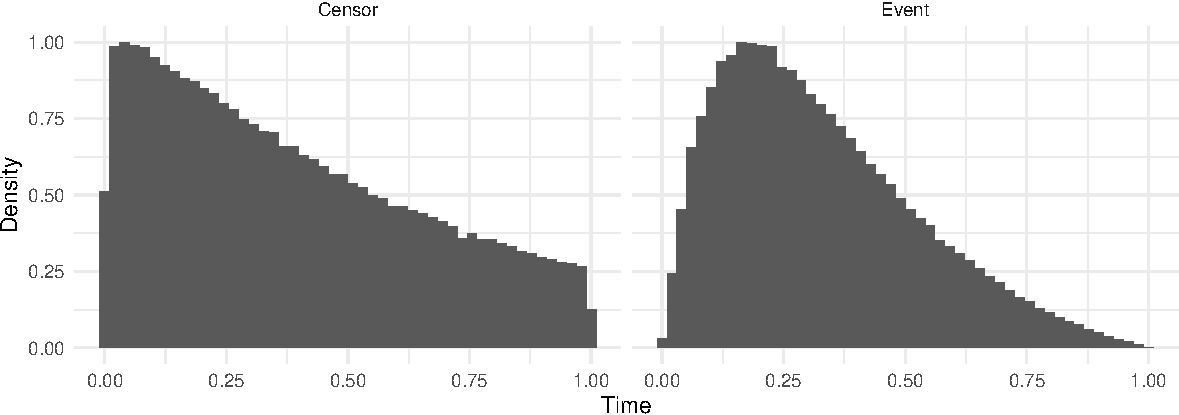
\includegraphics{ProgressReport_files/figure-latex/SimDataDensity-1.pdf}

\subsection{Model overfit}\label{model-overfit}

\subsubsection{Incident/Dynamic AUC}\label{incidentdynamic-auc}

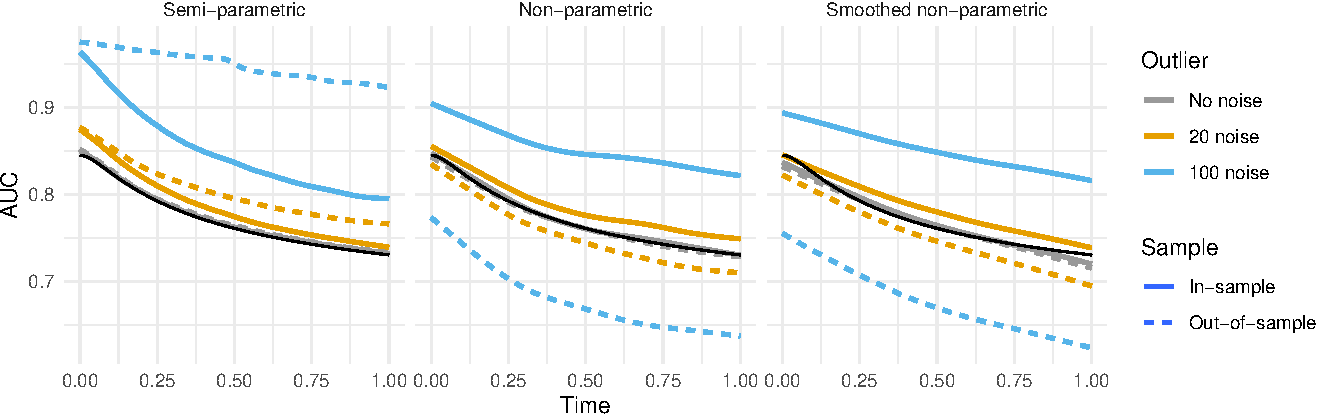
\includegraphics{ProgressReport_files/figure-latex/fig_tv_auc_noise-1.pdf}

\subsubsection{Spread of Incident/Dynamic
AUC}\label{spread-of-incidentdynamic-auc}

\begin{itemize}
\tightlist
\item
  with the continuous censoring distribution, at some cases the
  non-parametric values ended up as NA. Also, The semi-parametric when
  can go over (0, 1) range.
\end{itemize}

\begin{verbatim}
## Warning: Removed 146 rows containing non-finite outside the scale range
## (`stat_boxplot()`).
\end{verbatim}

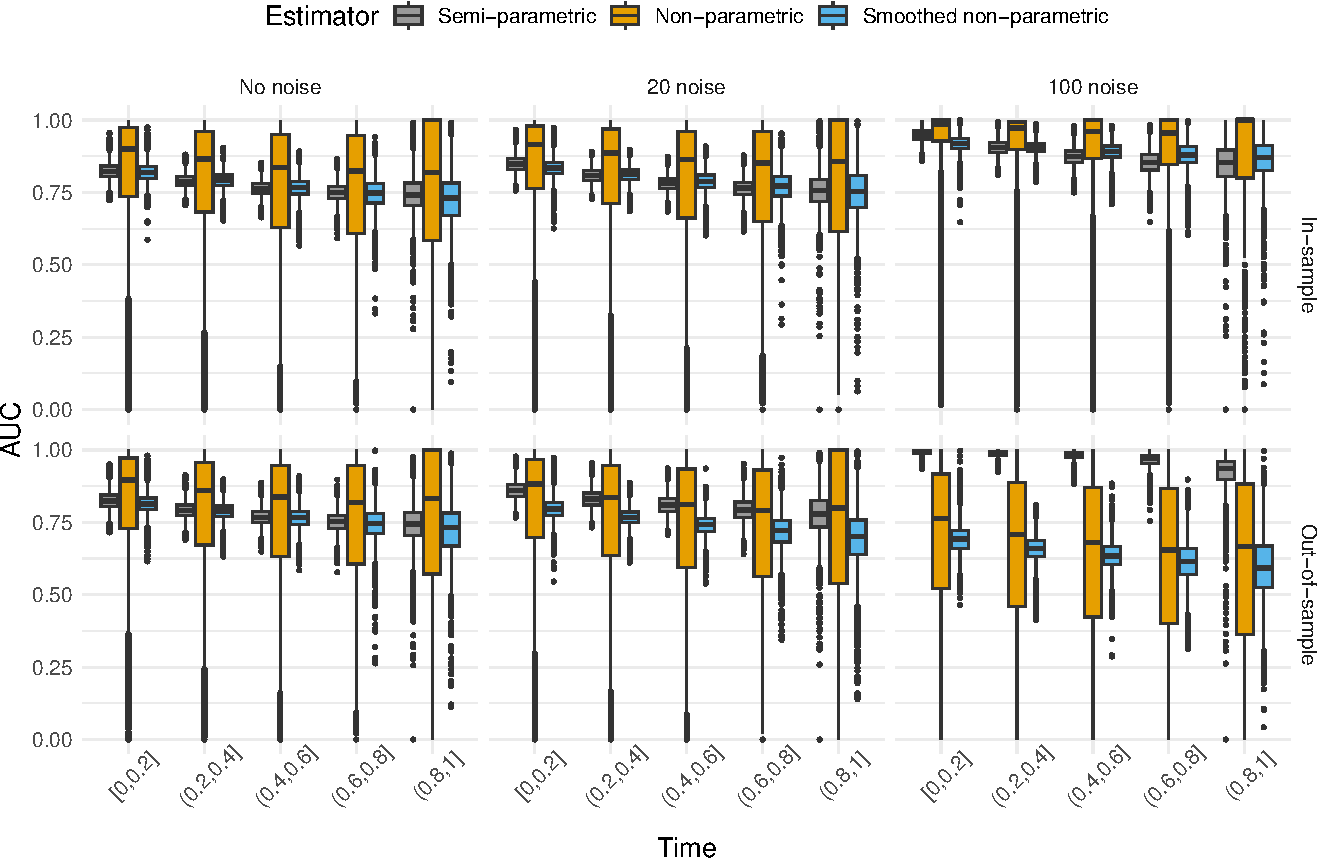
\includegraphics{ProgressReport_files/figure-latex/fig_tvauc_box_ovefit-1.pdf}

\subsubsection{Concordance}\label{concordance}

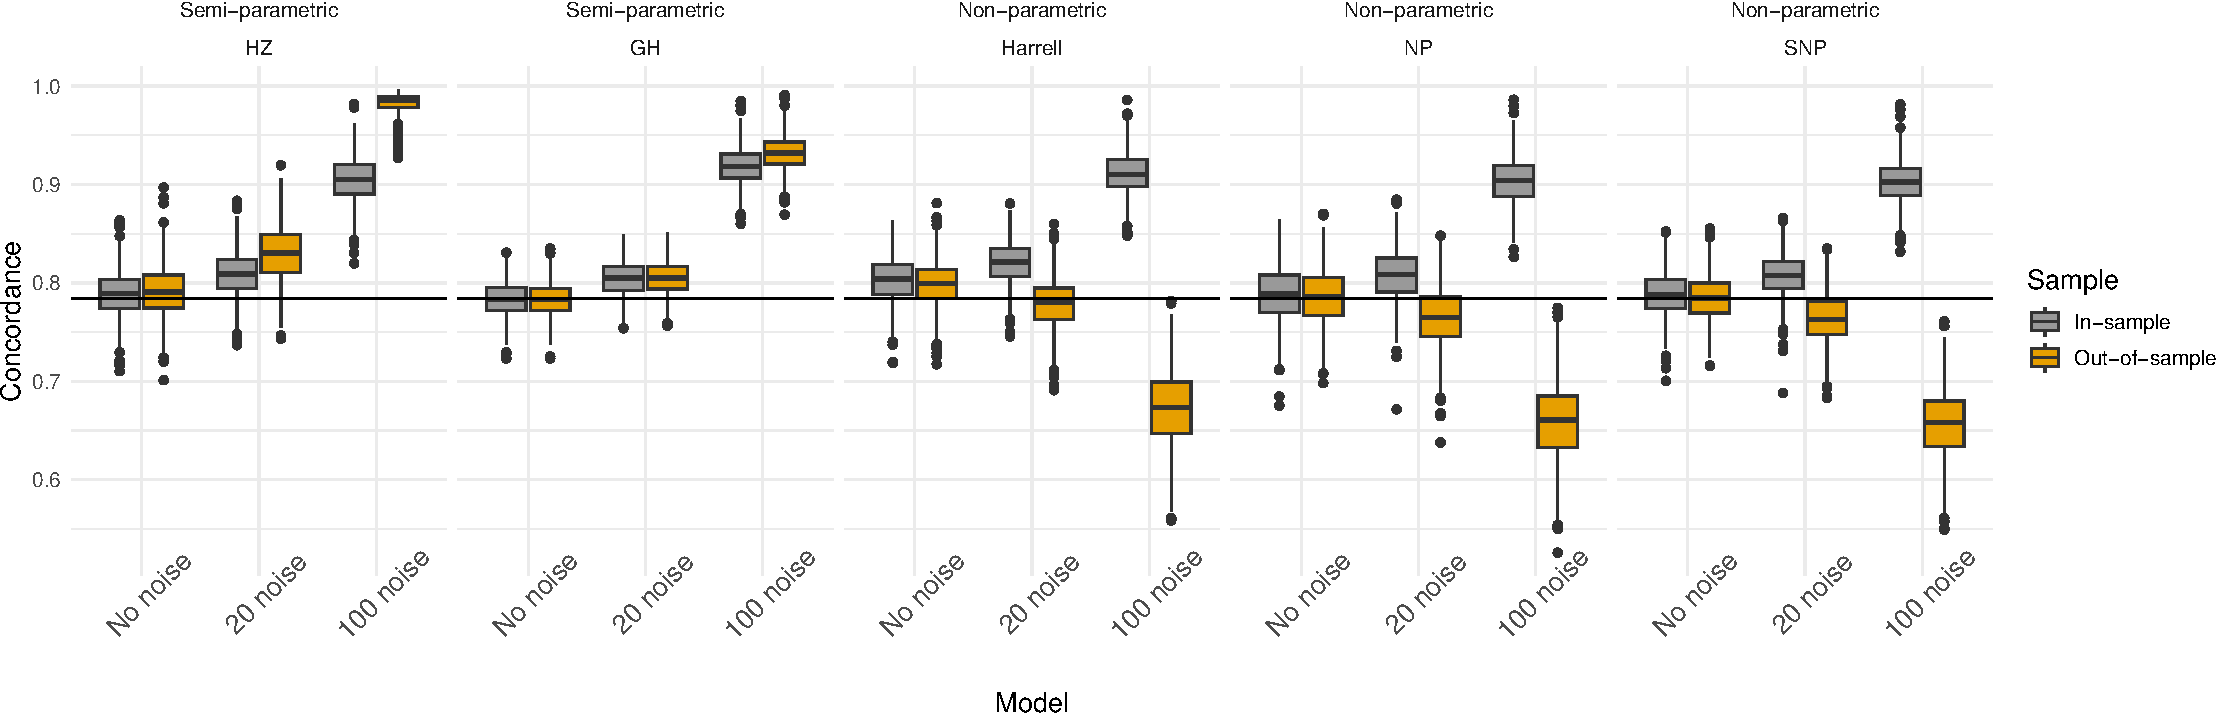
\includegraphics{ProgressReport_files/figure-latex/fig_c_noise-1.pdf}

\subsection{Data contamination}\label{data-contamination}

\begin{itemize}
\tightlist
\item
  Data contamination is introduced by adding outliers to test datasets
  (not noise in the model)
\item
  Within each simulation, we investiage two scenarios:
\end{itemize}

\begin{enumerate}
\def\labelenumi{\arabic{enumi}.}
\tightlist
\item
  10\% contaminated subjects, N(5, 1)
\item
  10\% contaminated subjects, N(0, 5)
\end{enumerate}

\subsubsection{Incident/Dynamic AUC}\label{incidentdynamic-auc-1}

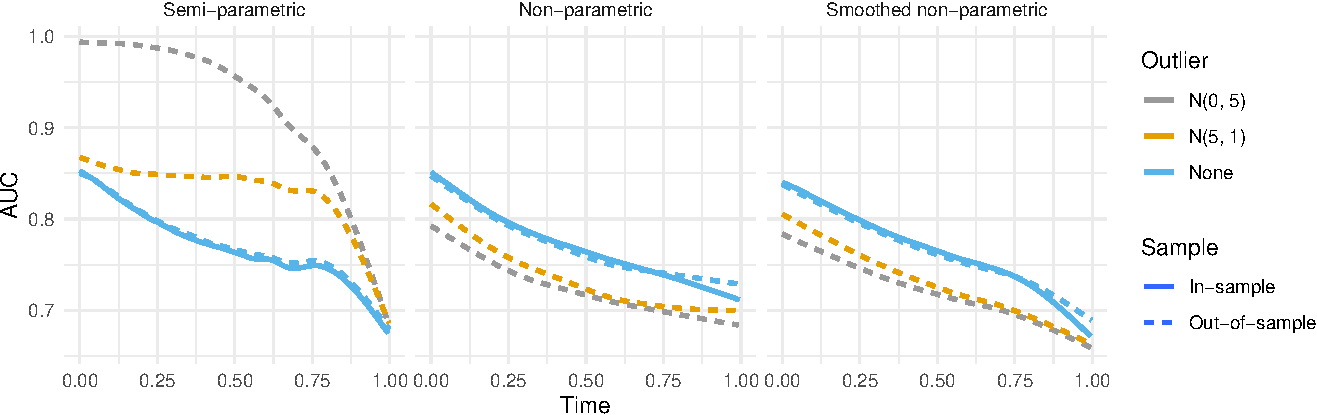
\includegraphics{ProgressReport_files/figure-latex/fig_tv_auc_contam-1.pdf}

\subsubsection{Spread of Incident/Dynamic
AUC}\label{spread-of-incidentdynamic-auc-1}

\begin{verbatim}
## Warning: Removed 87 rows containing non-finite outside the scale range
## (`stat_boxplot()`).
\end{verbatim}

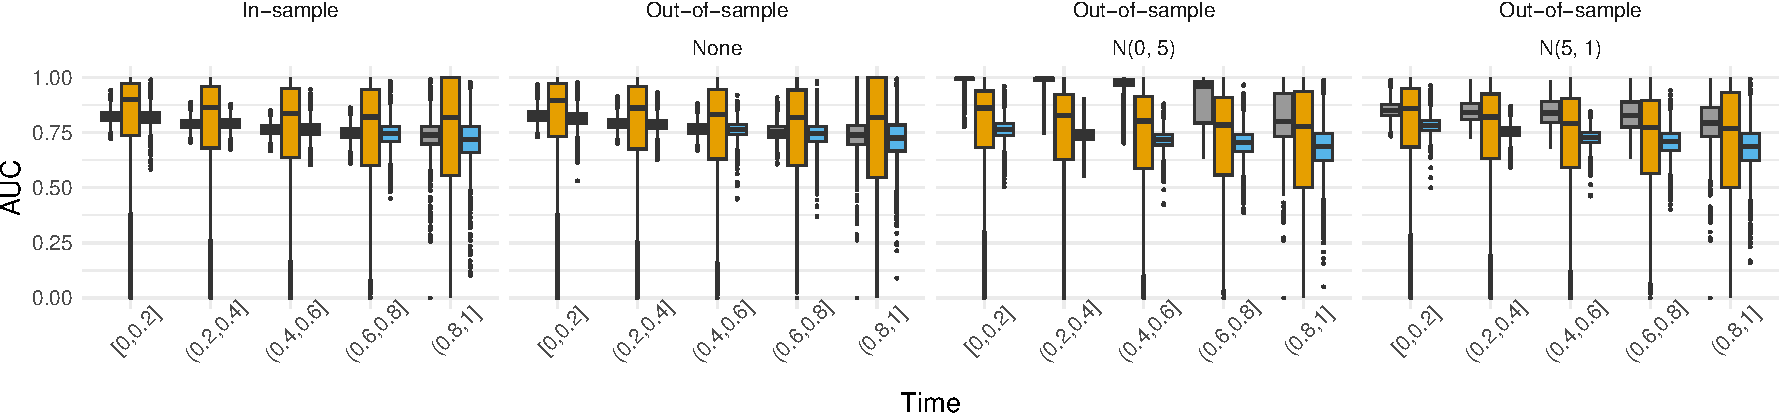
\includegraphics{ProgressReport_files/figure-latex/fig_tvauc_box_contam-1.pdf}

\subsubsection{Concordance}\label{concordance-1}

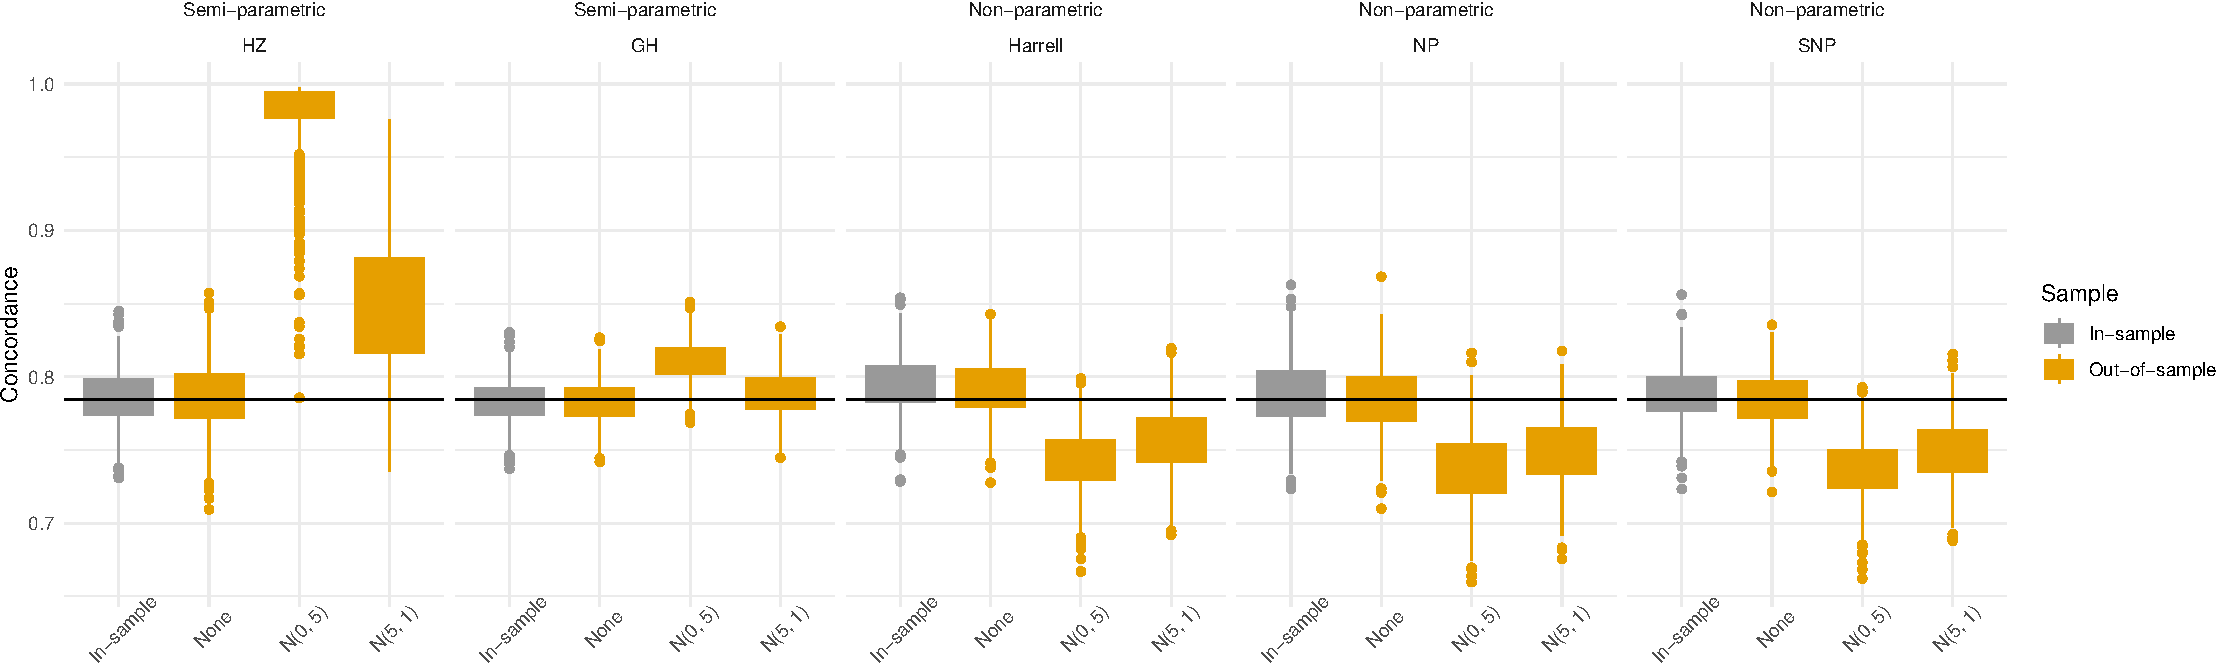
\includegraphics{ProgressReport_files/figure-latex/fig_c_contam-1.pdf}

\section{Case Study}\label{case-study}

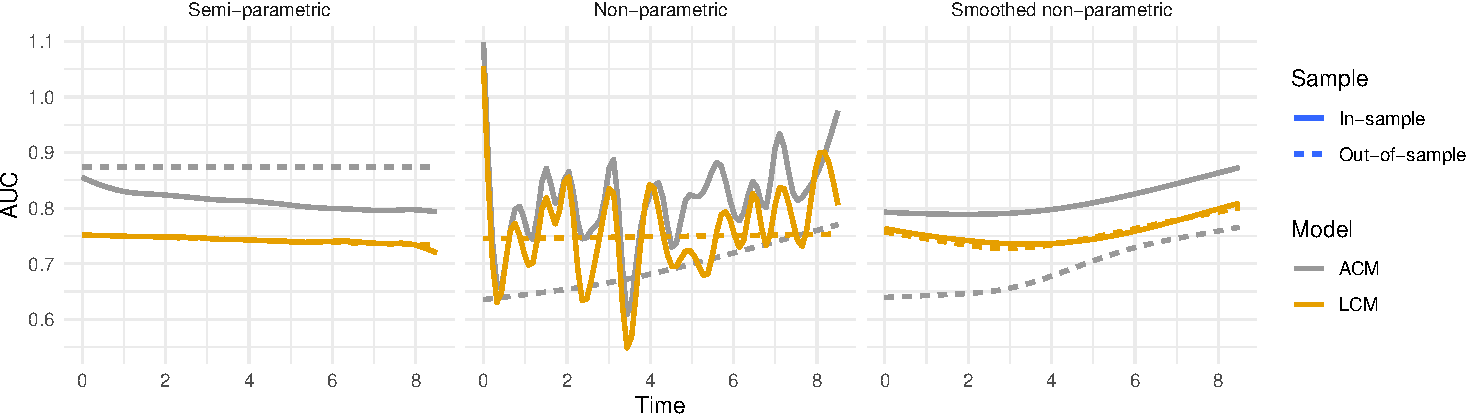
\includegraphics{ProgressReport_files/figure-latex/appl_auc-1.pdf}

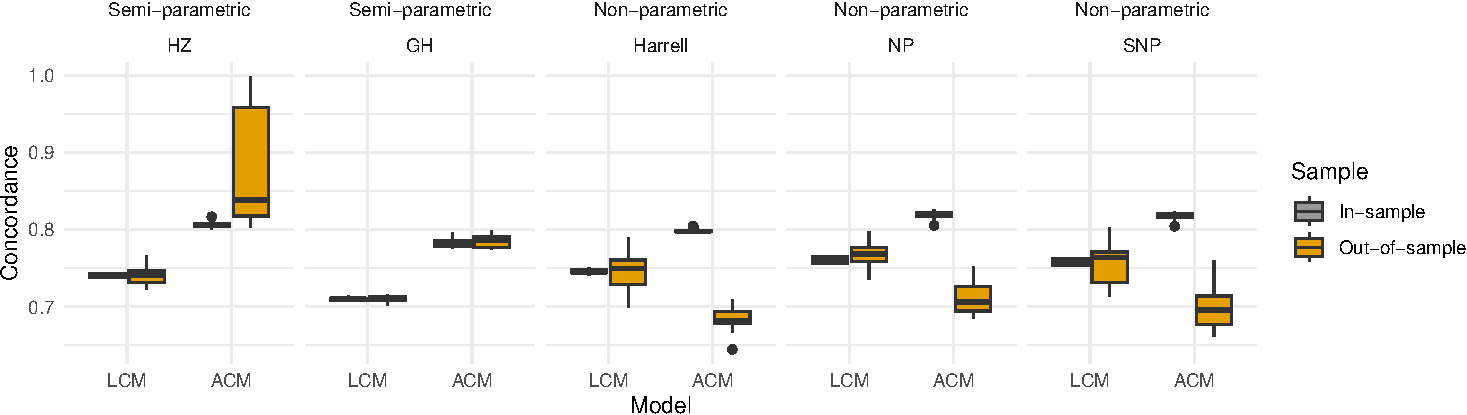
\includegraphics{ProgressReport_files/figure-latex/appl_c-1.pdf}
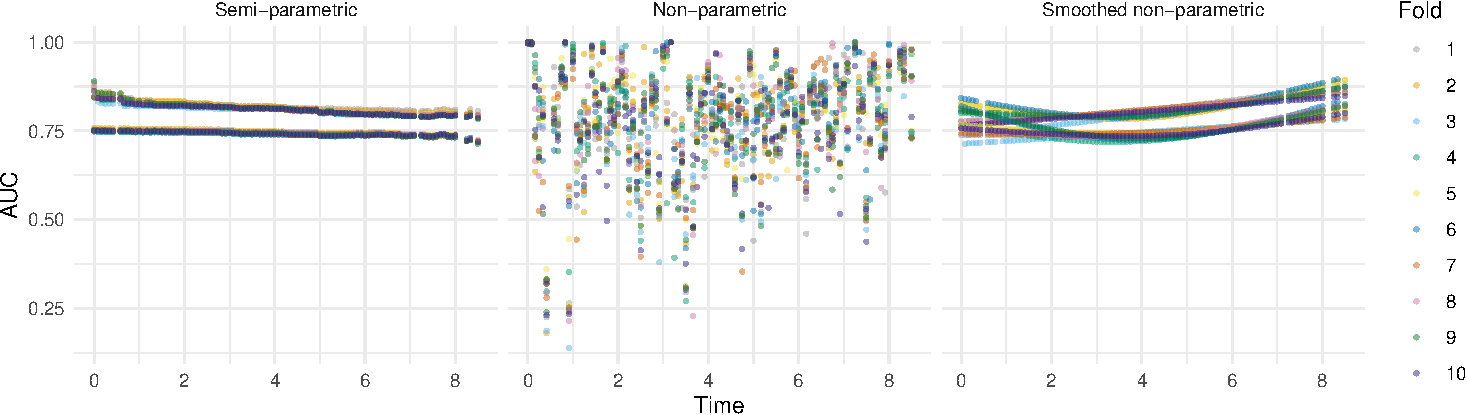
\includegraphics{ProgressReport_files/figure-latex/auc_t_scatter-1.pdf}

\section{Summary table}\label{summary-table}

\begin{longtable}[t]{llll}
\toprule
Estimator & Bias & Variavility & Out-of-sample behavior\\
\midrule
\addlinespace[0.3em]
\multicolumn{4}{l}{\textbf{Time-dependent AUC}}\\
\hspace{1em}Semi-parametric & Unbiased & Low & Over-optimistic\\
\hspace{1em}Non-parametric & Unbiased & High & \vphantom{1} Appropriate\\
\hspace{1em}Smoothed non-parametric & Slightly biased & Low & Appropriate\\
\addlinespace[0.3em]
\multicolumn{4}{l}{\textbf{Concordance (semi-parametric)}}\\
\hspace{1em}Heagerty-Zheng & Unbiased & Low & Over-optimistic\\
\hspace{1em}Gonen-Heller & Unbiased & Low & Over-optimistic\\
\addlinespace[0.3em]
\multicolumn{4}{l}{\textbf{Concordance (non-parametric)}}\\
\hspace{1em}Non-parametric & Unbiased & High & Appropriate\\
\hspace{1em}Smoothed non-parametric & Unbiased & Low & Appropriate\\
\hspace{1em}Harrell & Biased upwards & Low & Appropriate\\
\bottomrule
\end{longtable}

\section{Appendix}\label{appendix}

\begin{itemize}
\tightlist
\item
  Use one simulated dataset to investigate the weight estimates used in
  the Heagerty-Zheng estimator of Incident/Dynamic AUC
\end{itemize}

\subsection{Model overfit}\label{model-overfit-1}

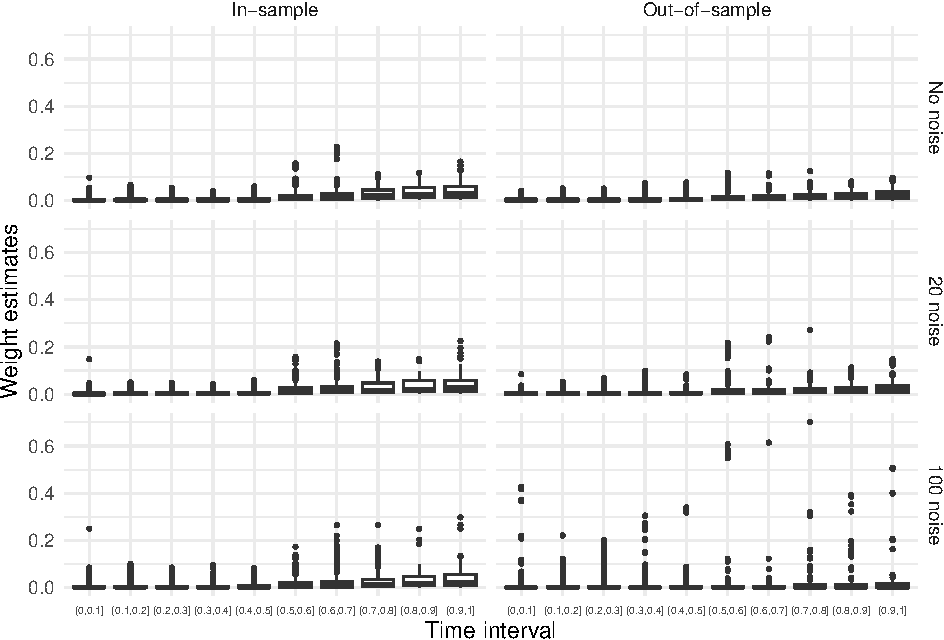
\includegraphics{ProgressReport_files/figure-latex/boxp_wt_noise-1.pdf}

\subsection{Data contamination}\label{data-contamination-1}

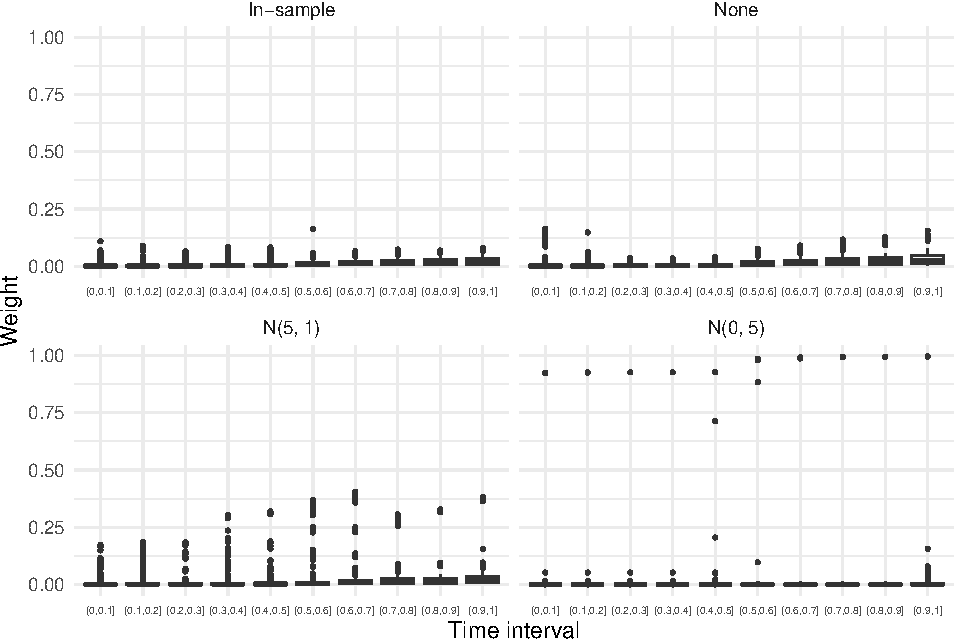
\includegraphics{ProgressReport_files/figure-latex/boxp_wt_contam-1.pdf}

\end{document}
